\documentclass[paper=a4, fontsize=11pt]{scrartcl} 

\usepackage[T1]{fontenc} 
\usepackage[english]{babel}
\usepackage{amsmath,amsfonts,amsthm}

\usepackage{lipsum}

\usepackage{graphicx}
\usepackage{float}
  \floatplacement{figure}{H}
  \floatplacement{table}{H}
  
\usepackage{sectsty} 
\allsectionsfont{\centering \normalfont\scshape} 

\usepackage{fancyhdr} % Custom headers and footers
\pagestyle{fancyplain} % Makes all pages in the document conform to the custom headers and footers
\fancyhead{} % No page header - if you want one, create it in the same way as the footers below
\fancyfoot[L]{} % Empty left footer
\fancyfoot[C]{} % Empty center footer
\fancyfoot[R]{\thepage} % Page numbering for right footer
\renewcommand{\headrulewidth}{0pt} % Remove header underlines
\renewcommand{\footrulewidth}{0pt} % Remove footer underlines
\setlength{\headheight}{13.6pt} % Customize the height of the header

\usepackage[labelformat=empty]{caption}
\usepackage{color}
\usepackage{listings}
\lstset{ %
language=bash,                % choose the language of the code
basicstyle=\footnotesize,       % the size of the fonts that are used for the code
numbers=left,                   % where to put the line-numbers
numberstyle=\footnotesize,      % the size of the fonts that are used for the line-numbers
stepnumber=1,                   % the step between two line-numbers. If it is 1 each line will be numbered
numbersep=5pt,                  % how far the line-numbers are from the code
backgroundcolor=\color{white},  % choose the background color. You must add \usepackage{color}
showspaces=false,               % show spaces adding particular underscores
showstringspaces=false,         % underline spaces within strings
showtabs=false,                 % show tabs within strings adding particular underscores
frame=single,           % adds a frame around the code
tabsize=2,          % sets default tabsize to 2 spaces
captionpos=b,           % sets the caption-position to bottom
breaklines=true,        % sets automatic line breaking
breakatwhitespace=false,    % sets if automatic breaks should only happen at whitespace
escapeinside={\%*}{*)}          % if you want to add a comment within your code
}
\usepackage{hyperref}


\numberwithin{equation}{section} % Number equations within sections (i.e. 1.1, 1.2, 2.1, 2.2 instead of 1, 2, 3, 4)
\numberwithin{figure}{section} % Number figures within sections (i.e. 1.1, 1.2, 2.1, 2.2 instead of 1, 2, 3, 4)
\numberwithin{table}{section} % Number tables within sections (i.e. 1.1, 1.2, 2.1, 2.2 instead of 1, 2, 3, 4)

\setlength\parindent{0pt} % Removes all indentation from paragraphs - comment this line for an assignment with lots of text

%----------------------------------------------------------------------------------------
%	TITLE SECTION
%----------------------------------------------------------------------------------------

\newcommand{\horrule}[1]{\rule{\linewidth}{#1}} % Create horizontal rule command with 1 argument of height

\title{	
\normalfont \normalsize 
\textsc{Computational Science - ITB} \\ [25pt] % Your university, school and/or department name(s)
\horrule{0.5pt} \\[0.4cm] % Thin top horizontal rule
\small  Pengenalan Sains Komputasi - Spreading Fire\\ % The assignment title
%\horrule{2pt} \\[0.5cm] % Thick bottom horizontal rule
}

\author{\small{Ridlo W. Wibowo || 20912009}} % Your name

\date{\normalsize\today} % Today's date or a custom date

\begin{document}

\maketitle % Print the title

\large \textbf{Problem.}\\
Develop a fire simulation in which every cell in a $17 \times 17$ grid has a tree and only the middle cell's tree is on fire initially. Do not consider the possibility of lightning or tree growth. The simulation should have a parameter for burnProbability, which is the probability of a tree adjacent to a burning tree catches fire. The function should return the percent of the forest burned. The program should run eight experiments with burnProbability = 10\%, 20\%, 30\%,..., and 90\% and should conduct each experiment 10 times. Also, have the code determine the average percent burned for each probability. Plot the data and fit a curve to the data. Discuss the results (Shodor, Fire).

\vspace{2cm}
\large \textbf{Documentation.}\\
Program dibuat sesuai kasus di atas tapi dengan memperhitungkan 8 arah/posisi grid untuk mengubah kondisi suatu grid, juga menggunakan \textit{periodic boundary} sebagai batas grid. Program dibuat dalam bahasa C++ dan OpenGL untuk membuat animasinya.\\

\textit{\textbf{Program}}
\lstset{frameround=fttt}
\begin{lstlisting}
// Copyleft (c) Ridlo W. Wibowo
// Simple Spreading Fire
// Ref: Tharindra Galahena Code, game_of_life cellular automata
#include <iostream>
#include <cstdlib>
#include <ctime>
#include <iostream>
#include <stdlib.h>
#include <GL/gl.h>
#include <GL/glut.h>
#include <fstream>
#include <time.h>

#define MAX 17

using namespace std;

int grid [MAX][MAX];
int grid2[MAX][MAX];
bool f = false;
int tpm = 200;
double burnProb = 0.4;

double unirand(){ return (double)rand()/(double)RAND_MAX;}

void inisiasi();

void menu(int t){
	tpm = t;
	glutPostRedisplay();
}

void printm(){
    int m=0;
    ofstream out("fire.txt");
    for (int i=0;i<MAX;i++){
        for (int j=0;j<MAX;j++){
            if (grid[i][j] == 1){ m++;}
            out << grid[i][j] << " ";}
        out << "\n";}
    out.close();
    cout << "tree = " << m << endl;
    cout << "persentase = " << (double)m*100./((double)MAX*MAX) << endl;
}

int check(int i, int j){
    // with periodic boundary 
    int s = 0;
	i += MAX;
	j += MAX;
    if (grid[i%MAX][j%MAX] == 1){
	    if(grid[(i - 1)%MAX][(j - 1)%MAX] == 2 && unirand() < burnProb){ s++;}
	    if(grid[(i - 1)%MAX][(j    )%MAX] == 2 && unirand() < burnProb){ s++;} 
	    if(grid[(i - 1)%MAX][(j + 1)%MAX] == 2 && unirand() < burnProb){ s++;}
	
	    if(grid[(i    )%MAX][(j - 1)%MAX] == 2 && unirand() < burnProb){ s++;} 
	    if(grid[(i    )%MAX][(j + 1)%MAX] == 2 && unirand() < burnProb){ s++;}
	
	    if(grid[(i + 1)%MAX][(j - 1)%MAX] == 2 && unirand() < burnProb){ s++;} 
	    if(grid[(i + 1)%MAX][(j    )%MAX] == 2 && unirand() < burnProb){ s++;} 
	    if(grid[(i + 1)%MAX][(j + 1)%MAX] == 2 && unirand() < burnProb){ s++;}

        return s;
	}
    else if (grid[i%MAX][j%MAX] == 2){return 999;}
    else{ return 888;}	
}

void copy(){
	for(int i = 0; i < MAX; i++){
		for(int j = 0; j < MAX; j++){
			grid[i][j] = grid2[i][j];
		}
	}
}

void spread(){ // update
	for(int i = 0; i < MAX; i++){
		for(int j = 0; j < MAX; j++){
            int s = check(i, j);
            if (s == 0){ grid2[i][j] = 1;} // ada pohon dan gak kebakar
            if (s > 0 && s < 9){ grid2[i][j] = 2;} // pohon terbakar
            if (s == 999){ grid2[i][j] = 0;} // udah kebakar jadi empty
            if (s == 888){ grid2[i][j] = 0;} // tetep empty
		}
	}
	copy();
}

void par(float x1, float x2, float y1, float y2, int val){
	if (val == 0){glColor3f(1.0, 1.0, 1.0);}
    else if(val == 1){ glColor3f(0.0, 1.0, 0.0);}
    else{glColor3f(1.0, 0.0, 0.0);}

	glBegin(GL_QUADS);
	
	glVertex3f(x1, y1, 0.0);
	glVertex3f(x2, y1, 0.0);
	glVertex3f(x2, y2, 0.0);
	glVertex3f(x1, y2, 0.0);

	glEnd();
}

void display(void)
{
	glClear(GL_COLOR_BUFFER_BIT | GL_DEPTH_BUFFER_BIT);
	glMatrixMode(GL_MODELVIEW);
	glLoadIdentity ();

	glTranslatef(0.0, 0.0, -22.0);
	
	for(int i = 0; i < MAX; i++){
		for(int j = 0; j < MAX; j++){
				par(-6.0 + 0.7 * j + 0.1,
					-6.0 + 0.7 * (j + 1),
					6.0 - 0.7 * i + 0.1,
					6.0 - 0.7 * (i - 1),
                    grid[i][j]);
		}
	}
	
	glutSwapBuffers();
}

void myIdleFunc(int a) {
	spread();
	glutPostRedisplay();
	if(f) glutTimerFunc(tpm, myIdleFunc, 0);
}

void inisiasi(){
	for (int i=0;i<MAX;i++){
        for (int j=0;j<MAX;j++){
            grid2[i][j] = 1;
        }
    }
    grid2[8][8] =  2;

    copy();
}

void keyboard(unsigned char key, int x, int y){
	if(key == 27) {		
		exit(0);	
	}else if((char)key == 'a'){
		if(!f) glutTimerFunc(tpm, myIdleFunc, 0);
		f = true;
	}else if((char)key == 's'){
		spread();
		glutPostRedisplay();
	}else if((char)key == 'd'){
		f = false;
	}else if((char)key == 'f'){
		inisiasi();
        f = false;
		glutPostRedisplay();
	}else if((char)key == 'p'){
        f = false;
        printm();
    }

}

void init(){
	glEnable(GL_DEPTH_TEST);
	glEnable(GL_COLOR_MATERIAL);

	glEnable(GL_LIGHTING);
	glEnable(GL_LIGHT0);
	glEnable(GL_NORMALIZE);
	glShadeModel(GL_SMOOTH);	
	glLoadIdentity ();
	glOrtho(-1.0, 1.0, -1.0, 1.0, -1.0, 1.0);

	GLfloat acolor[] = {1.4, 1.4, 1.4, 1.0};
	glLightModelfv(GL_LIGHT_MODEL_AMBIENT, acolor);
}

void Reshape(int w, int h){
    glViewport(0, 0, w, h);
    glMatrixMode(GL_PROJECTION); 
	glLoadIdentity();
	gluPerspective(45.0, (float)w/(float)h, 0.1, 200.0);
}

int main(int argc, char** argv){
    cout << "Input burnProbablity : "; cin >> burnProb;
	srand(time(NULL));
    inisiasi();
	
	glutInit(&argc,argv);
	glutInitDisplayMode ( GLUT_DOUBLE | GLUT_RGB | GLUT_DEPTH);
	glutInitWindowSize(700,700);
	glutInitWindowPosition(500,0);
	glutCreateWindow("Spreading Fire");
	glutCreateMenu(menu);

	glutAddMenuEntry( "20",  20);
	glutAddMenuEntry( "40",  40);
	glutAddMenuEntry( "60",  60);
	glutAddMenuEntry("100", 100);
	glutAddMenuEntry("150", 150);
	glutAddMenuEntry("200", 200);
	
	glutAttachMenu(GLUT_RIGHT_BUTTON);
	init();
	glutReshapeFunc(Reshape);
	glutKeyboardFunc(keyboard);
	glutDisplayFunc(display);
	
	glutMainLoop();
	return 0;
}
\end{lstlisting}

%\vspace{2cm}
\newpage
Setelah program dijalankan dapat dilakukan beberapa hal:
\begin{itemize}
\item input burnProb, input dari terminal (kemudian layar simulasi muncul)
\item tombol a = run simulasi otomatis
\item tombol s = run simulasi per step
\item tombol d = pause simulasi
\item tombol f = restart simulasi
\item tombol p = print kondisi (persen terbakar dan file berisi matriksnya)
\item tombol ESC = stop, exit
\item klik kanan pada layar simulasi, lalu pilih kecepatan simulasi (untuk kasus tombol a)
\end{itemize}
belum terbakar, sedang terbakar, dan sudah terbakar ditunjukkan dengan warna hijau, merah, dan putih. Contoh animasi dapat dilihat di \url{http://astrokode.wordpress.com/2012/11/28/spreading-fire-simulation-v01-with-opengl/}.\\

Screenshot:
\begin{figure}
	\centering
	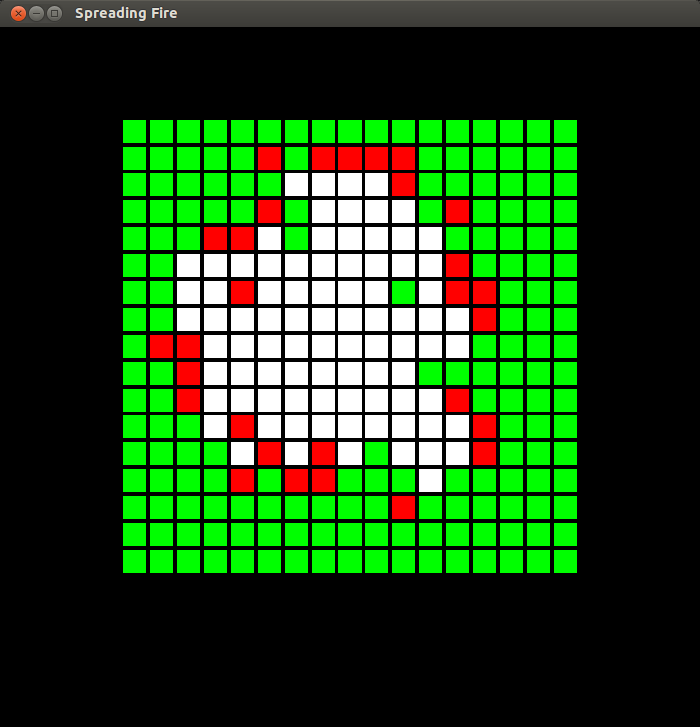
\includegraphics[width=0.6\textwidth]{spreadingFire.png}
	\caption{Screenshot layar simulasi.}
\end{figure}

\newpage
Hasil run untuk beberapa \textit{burnProbablity}:
\begin{table}[ht]
\begin{tabular}{c c}
\hline
\textit{burnProb} & average \% burned after 10$\times$ run \\ [0.5ex]
\hline 
0.1 & 1.007 \\
0.2 & 15.743 \\
0.3 & 80.657 \\
0.4 & 97.647 \\
0.5 & 99.723 \\
0.6 & 99.931 \\
0.7 & 100.0 \\
0.8 & 100.0 \\
0.9 & 100.0 \\ [1ex]
\hline 
\end{tabular}
\end{table}

Dengan melihat angka pada tabel di atas lalu dilakukan fitting menggunakan fungsi logistik sebagai berikut:
\begin{equation}
f(x) = \frac{100}{1 + A e^{-\lambda x}}
\end{equation}

menggunakan fitting nonlinear pada \textit{gnuplot} diperoleh: \\
(sebenarnya bisa diubah menjadi fitting linear karena nilai maksimum sudah diketahui \--- 100\%)\\
$ A = 2532.45 \pm 320.7 $\\
$ \lambda = 30.8436 \pm 0.482$
\begin{figure}
	\centering
	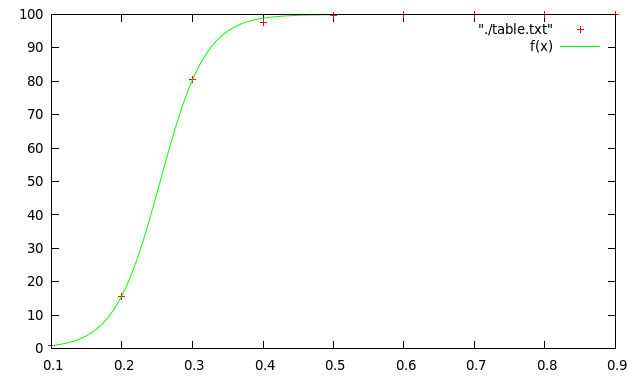
\includegraphics[width=0.6\textwidth]{plot.png}
	\caption{Plot data (+ merah) dan fitting menggunakan fungsi logistik (garis hijau).}
\end{figure}
 
\textbf{Diskusi}
\begin{enumerate}
\item Terjadi lonjakan nilai persentase terbakar untuk \textit{burnProb} antara 0.2 dan 0.3, ketika nilainya lebih besar dari itu, hampir semua grid pasti terbakar habis, jika kurang dari itu api susah menyebar (terdapat nilai kritis).
\item Bentuk fungsi logistik cocok untuk menggambarkan peristiwa ini.
\end{enumerate}

\end{document}














